\documentclass[conference]{IEEEtran}
\IEEEoverridecommandlockouts
% The preceding line is only needed to identify funding in the first footnote. If that is unneeded, please comment it out.
\usepackage{cite}
\usepackage{amsmath,amssymb,amsfonts}
\usepackage{algorithmic}
\usepackage{graphicx}
\usepackage{textcomp}
\usepackage{xcolor}
\def\BibTeX{{\rm B\kern-.05em{\sc i\kern-.025em b}\kern-.08em
    T\kern-.1667em\lower.7ex\hbox{E}\kern-.125emX}}
\begin{document}

\title{Dashcam for Traffic Object Detection\\ }

\makeatletter
\newcommand{\linebreakand}{%
  \end{@IEEEauthorhalign}
  \hfill\mbox{}\par
  \mbox{}\hfill\begin{@IEEEauthorhalign}
}
\makeatother

\def\Affiliation{ School of Electrical Engineering }
\def\Organization{Telkom University, Indonesia}
\def\CityCountry{Bandung, Indonesia}

\author{\IEEEauthorblockN{Aura Syafa Aprilia Radim}
\IEEEauthorblockA{\textit{\Affiliation } \\
\textit{\Organization}\\
\CityCountry \\
syafaaura@student.telkomuniversity.ac.id }
\and
\IEEEauthorblockN{Muchammad 'Irfan Chanif Rusydi}
\IEEEauthorblockA{\textit{\Affiliation } \\
\textit{\Organization}\\
\CityCountry \\
email address or ORCID}
\and
\IEEEauthorblockN{Surya Michrandi Nasution}
\IEEEauthorblockA{\textit{\Affiliation} \\
\textit{\Organization}\\
\CityCountry \\
email address or ORCID}
\linebreakand
% \IEEEauthorblockN{4\textsuperscript{th} Given Name Surname}
% \IEEEauthorblockA{\textit{dept. name of organization (of Aff.)} \\
% \textit{name of organization (of Aff.)}\\
% City, Country \\
% email address or ORCID}
% \and
\IEEEauthorblockN{Casi Setianingsih}
\IEEEauthorblockA{\textit{\Affiliation} \\
\textit{\Organization}\\
\CityCountry \\
email address or ORCID}
% \and
% \IEEEauthorblockN{6\textsuperscript{th} Given Name Surname}
% \IEEEauthorblockA{\textit{dept. name of organization (of Aff.)} \\
% \textit{name of organization (of Aff.)}\\
% City, Country \\
% email address or ORCID}
}

\maketitle

\begin{abstract}
Dashcam is a camera stored in a vehicle. This tool serves to record all events in front of the vehicle. Security and safety have become a major concern in various sectors, including transportation and public security. On the highway, traffic accidents caused by the driver's ignorance of objects around the vehicle are still a serious problem. In this study, the development of a simple dashcam built from an edge computer was carried out by combining the number of cameras. Image stitching is applied to combine images that have been collected by each camera. Next, object detection is carried out on the images that have been collected. The object detection system approach is carried out using YOLOv8 which is the latest variant of the YOLO series. This research is expected to be one step in the development of an Intelligent Transportation System that is in accordance with traffic conditions in Indonesia. The results obtained in testing using the system created exist using the configuration of 78000 datasets, 3332 data validation with 8 epochs, batch size 32, linear learning rate and SGD optimization. Results are best in the morning and afternoon. The program can recognize predefined objects. 
\end{abstract}

\begin{IEEEkeywords}
object detection, YOLOv8, dashcam
\end{IEEEkeywords}

\section{Introduction}
Security and safety have become a major concern in various sectors, including transportation and public security. On the highway, traffic accidents caused by the driver's ignorance of objects around the vehicle are still a serious problem. Smart and effective object detection technology is becoming increasingly important for monitoring traffic [1]. 

Video captures from dashcams usually only show one side according to the camera position. However, this results in a lack of information about nearby objects. To overcome this problem, this study tried a solution by using two cameras or cameras placed at different positions in the vehicle. By using more than one camera, diverse viewing angles can provide more complete information about objects around the vehicle. For example, the camera on the left side helps detect objects on the left, while the camera on the right side helps detect objects on the right. This approach is expected to provide more comprehensive results according to the actual situation in front of the vehicle.
Therefore, the study of the application of dual cameras to detect objects becomes very relevant and interesting. By optimizing the use of dual cameras, it is hoped that this technology will be able to provide effective solutions in increasing driver awareness and safety on the road. The application of dual cameras for object detection has the potential to reduce accident incidents, reduce the risk of collisions, and improve the safety of all road users. 

\section{Literature Review}

\subsection{Object Detection}
Object Detection is one of the important task in computer vision field, mainly dealing with detecting instances of visual object then categorize them into several classes \cite{b2}.
With this kind of identification and localization, object detection can be used to count objects in a scene and determine and track their precise locations, all while accurately labeling them.
Object detection has been widely used for face detection, vehicle detection, pedestrian counting, web images, security systems and driverless cars.
Within the past twenty years, object detection have been going through a lot of changes and development. Although it is commonly divided into two periods: "traditional object detection" and "deep learning based". In 2012, Krizhevsky et al. \cite{b3} proposed a deep convolutional network trained on a subset of ImageNet. 

This network, called AlexNet, was the first to demonstrate that convolutional neural networks (CNNs) could be trained effectively on large-scale datasets and used to achieve state-of-the-art object detection results.
A year later, Girshick et al. proposed a new object detection framework called R-CNN \cite{b4} because it used region proposals combined with CNNs to detect objects in images.
Since then, the field of object detection has been rapidly advancing, with new models, datasets, and techniques emerging in a rapid pace. 

\subsection{You Only Look Once (YOLO)}
With the born of AlexNet, YOLO \verb|(You Only Look Once)| model was introduced in 2015. Base YOLO model can achieve 45 frame per second. While the sameller version, Fast YOLO can achieve 155 frames per second.
YOLO outperform DPM and R-CNN on Picasso Dataset and People-Art Dataset \cite{b5}.

In the early period of making this paper, YOLOv7 was the latest version of YOLO. However,as January 2023, YOLOv8 was introduced by Ultralytics, the same software company that release YOLOv3 and YOLOv5. 
                                                                                                                                                                                                                                                                                                                                                                                                                                                                                                                    

\section{System Design}

\subsection{COCO Dataset}\label{AA}
The COCO dataset is a large-scale object detection, segmentation, and keypoint dataset.
In total, The Microsoft Common Objects in COntext contains 91 common object categories with 82 of them having more than 5,000 labeled instances \cite{b6}.
The first release of COCO Dataset was in 2014. In 2014, COCO Dataset has 83,000 image in train split and 41,000 image in validation split. 


\subsection{Dataset Filtering}
As mention earlier, COCO dataset contains 80 classes. However, we only need traffic related object classess.
Therefore, we filtered the dataset to only contain 12 classes. The classes are:
Car Truck Bus Motorcycle Bicycle Traffic Light Stop Sign Train Hydrant Cat Dog
The result is 78,663 images in training split with 12 classes. This amount of data was reduced from 122,125 images in original dataset. By reducing the dataset, our model expected to take less time to train.
Fig(1) shows the comparison of training session for 8 epoch between filtered dataset and original dataset.
\begin{figure}

\end{figure}

In addition, as shown in Fig1 and Fig2, the filtered dataset has lower GPU Utilization and Memory Utilization. This means that the filtered dataset is more efficient to train.
Thus allowing us to push model training further.
Metrics wise, the model trained using filtered dataset showed better result.


\subsection{Metrics}
For training and validation purposes, we focus on mAP (mean Average Precision), Precision, and recall. mAP is the average of AP (Average Precision) over all classes. AP is the area under the precision-recall curve.
We compare mAP averaged for IoU (Intersection over Union) thresholds from .50 to .95 with .05 increments (MS COCO standard metric, abbreviated as mAP50-95) and (PASCAL VOC metric, abbreviated as mAP50) \cite{b7}. 
Precision and Recall in  this experiment is a relative measure, because it depends on the threshold value.
Precision calculated by dividing True Positive by the sum of True Positive and False Positive. 


Recall calculated by dividing True Positive by the sum of True Positive and False Negative.


Threshold value determines whether the prediction is Positive or Negative. For example, if the threshold is 0.5, then the prediction is positive if the probability is greater than 0.5. Otherwise, the prediction is negative.\
Therefore, both Precision and Recall are relative to the threshold value and usually used in the form of Precision-Recall Curve.

\section{Experiments}


\subsection{Experimental Setup}
In this section, we will discuss about the experimental setup. We are using Pytorch as our deep learning framework in Python  3.
MNodel training was conducted on Geforce RTX 3090, 24 GB VIdeo RAM, 32GB RAM, Intel Core i3-12100 4 Core 8 Thread, running on Windows 10
Model inference and testing was performed on Macbook Air M1, and Jetson Nano 4GB. The camera used in this experiment  LifeCam Studio by Microsoft.

\subsection{Dataset}
As mention earlier, we are using COCO dataset. However, we filtered the dataset to only contain 12 classes. The classes are:
Car, Truck, Bus, Motorcycle, Bicycle, Traffic Light, Stop Sign, Train, Hydrant, Cat, Dog. The result is 78000 images with 12 classes.
For inference and real world testing, we gather our own data by recording traffic condition in Bandung, Indonesia. The data was recorded using camera mentioned earlier.

\subsection{Training}
Before we begin training process of our YOLOv8n-Traffic model with high number of epoch, we want to find the optimal hyperparamater configuration for our use case. We conducted various training configuration with 8 epoch.
We tried different batch size, learning rate, and optimizer. We use batch size 16 and 32. Fig(1) shows the result of training with different batch size. We can see that batch size 32 is better than batch size 16. Therefore, we use batch size 32 for our training.
We also tried using SGD and Adam optimizer.


\subsection{Real World Testing}
\begin{figure}[h]
    \centering
    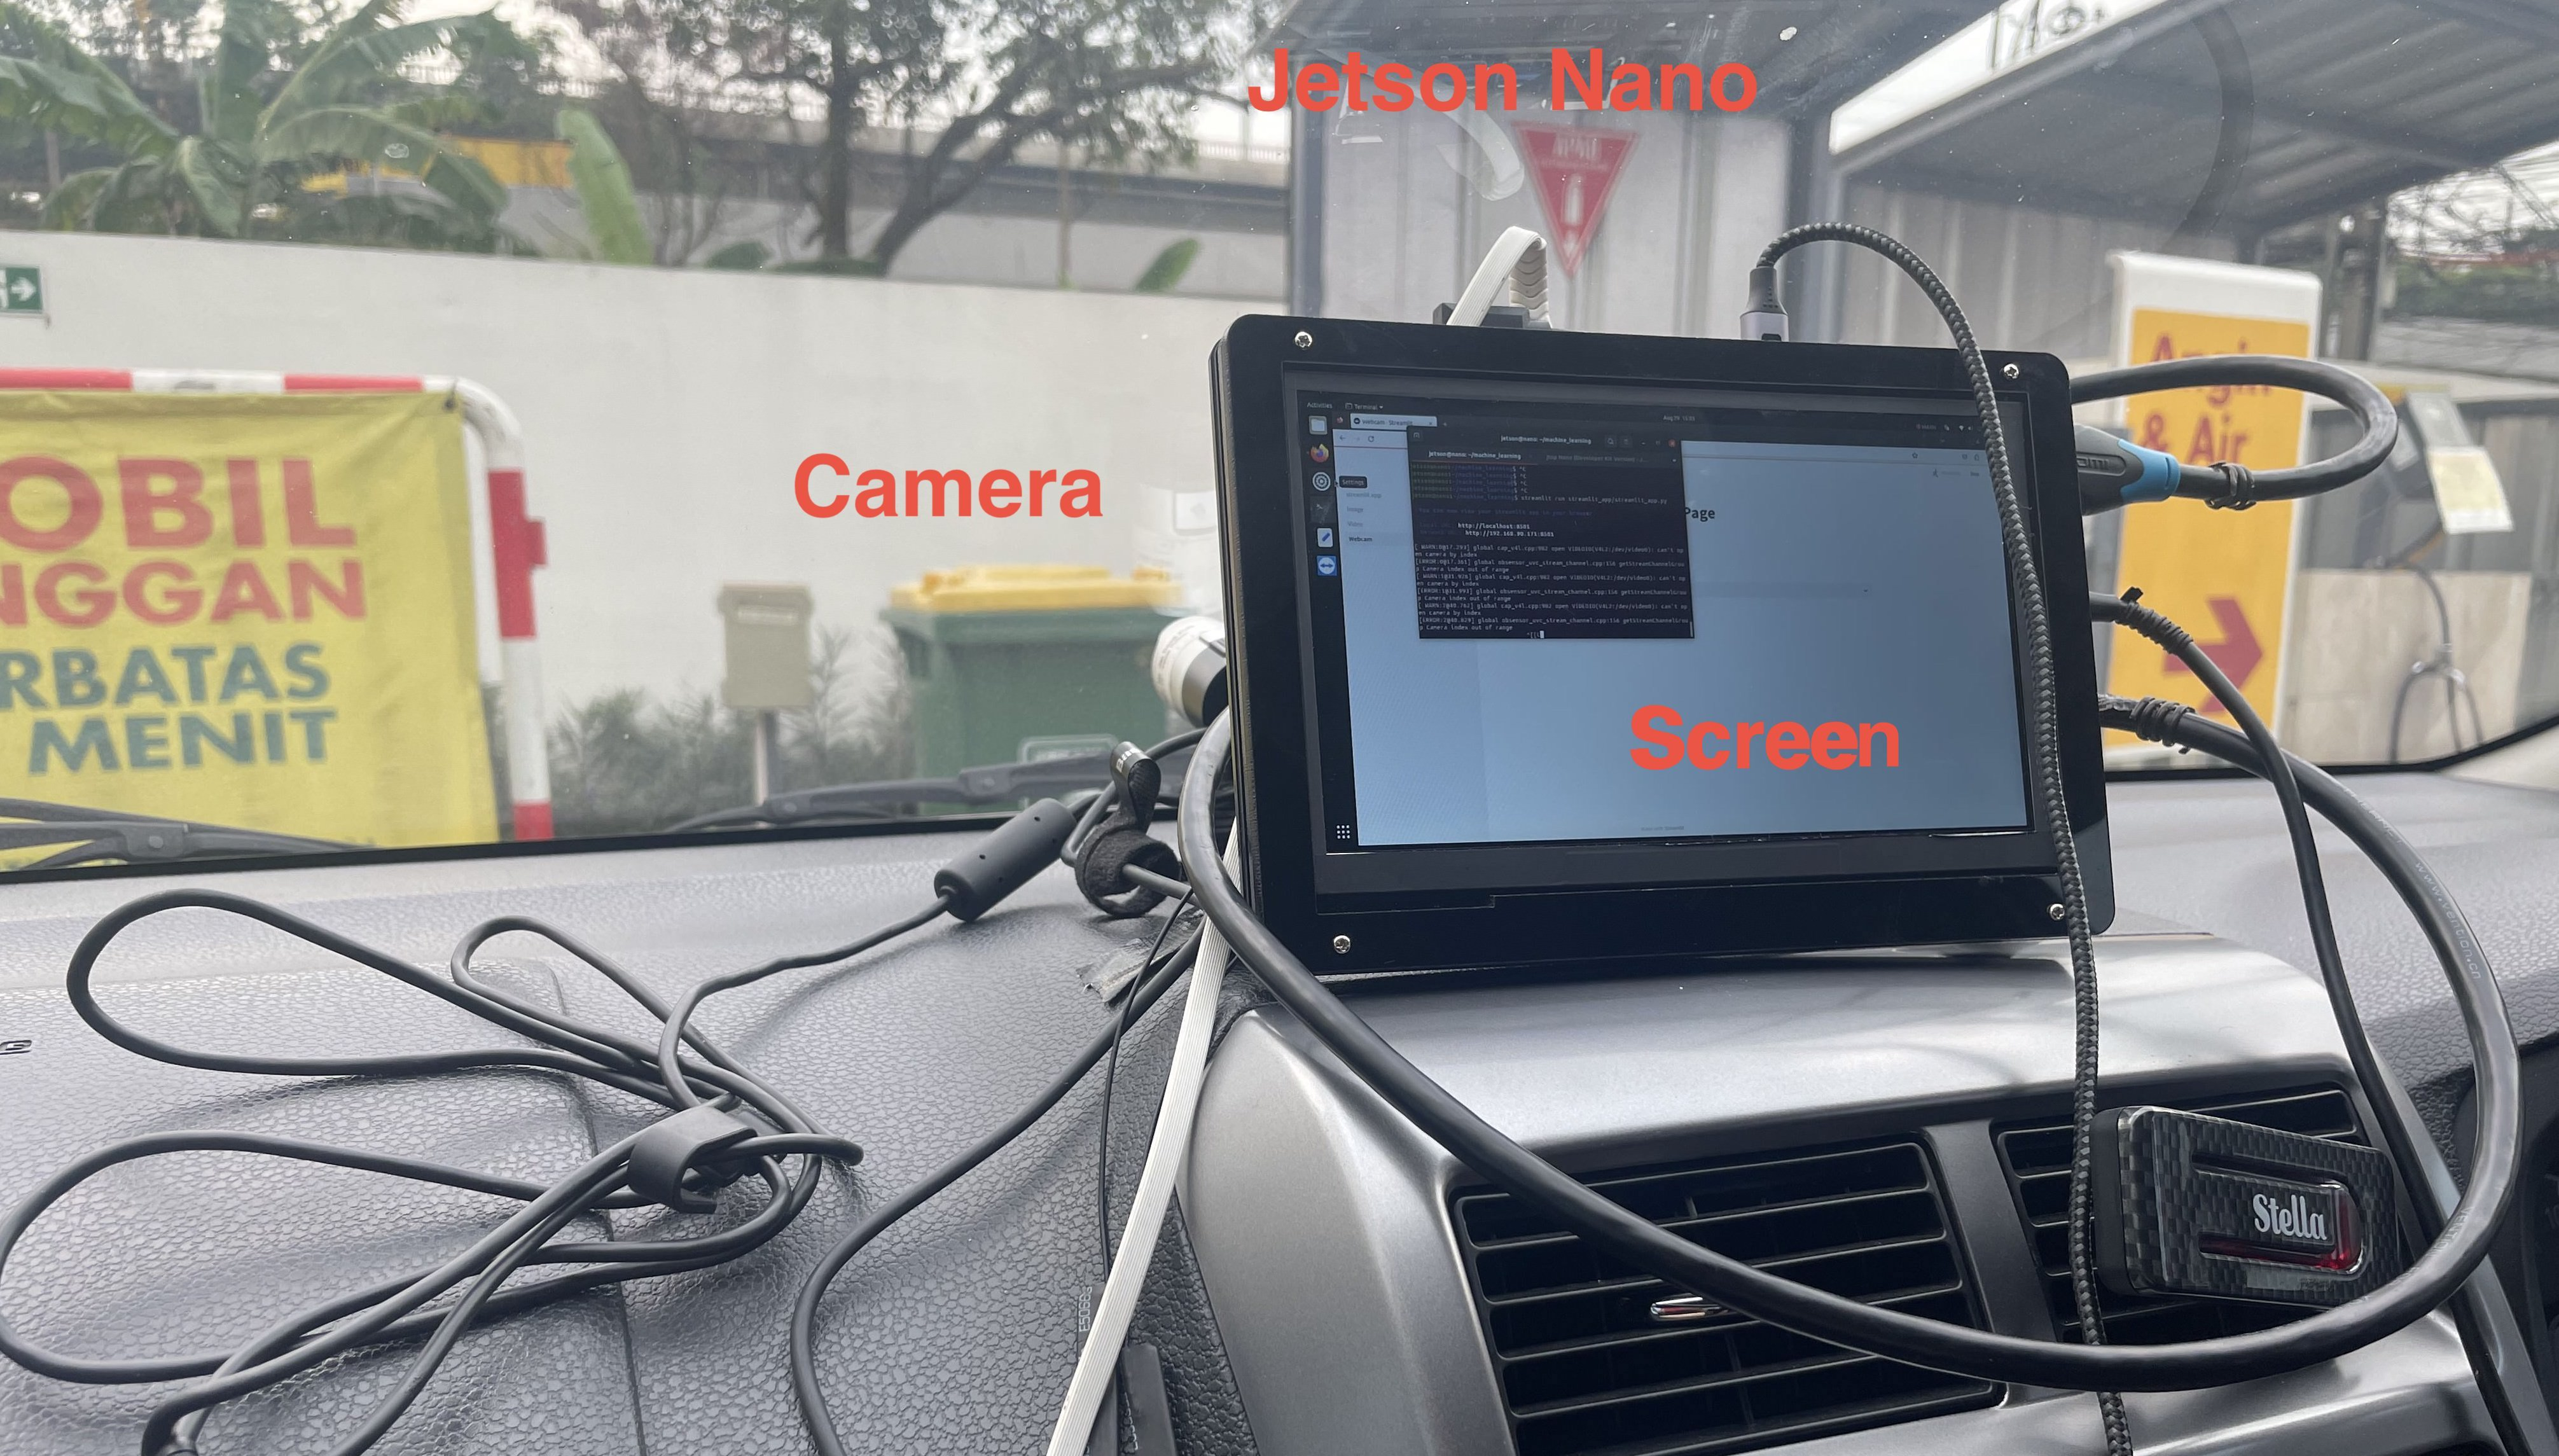
\includegraphics[width=0.25\textwidth]{mounted_camera_front_view.jpg}
    \caption{Front View}
    \label{fig:front_view}
\end{figure}

\begin{figure}
    \centering
    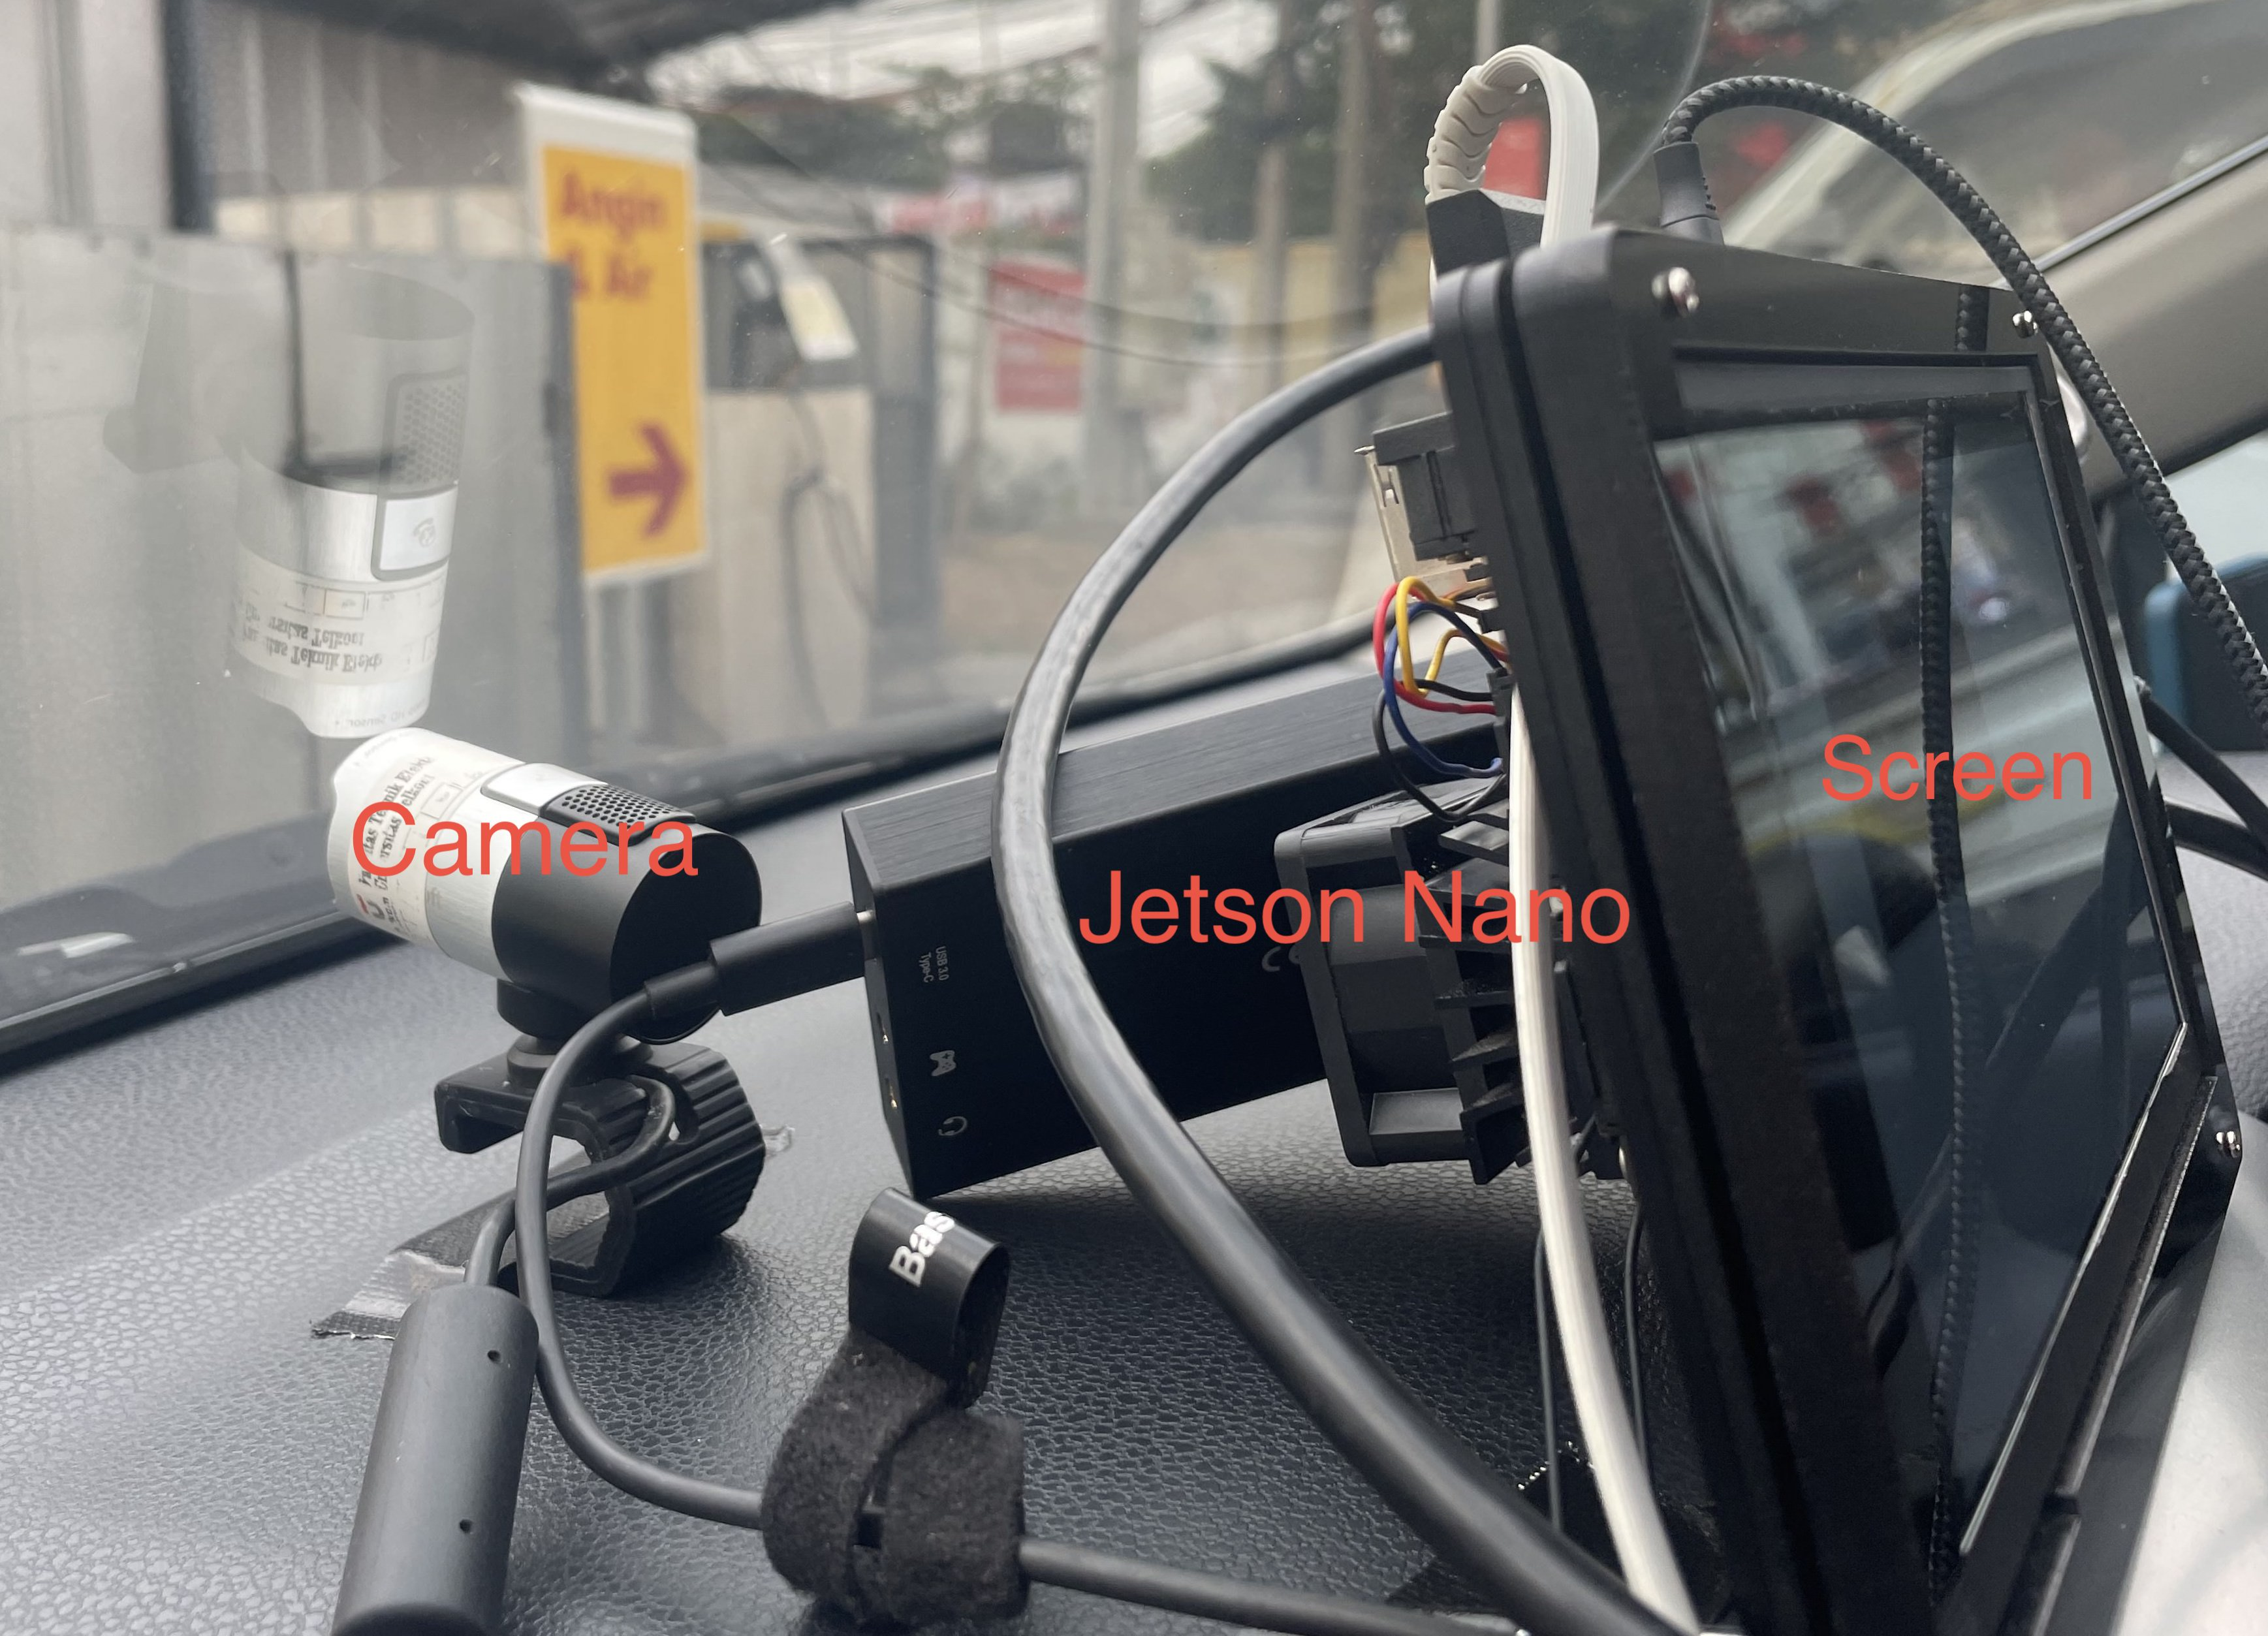
\includegraphics[width=0.25\textwidth]{mounted_camera_side_view.jpg}
    \caption{Side View}
    \label{fig:side_view}
\end{figure}
\section{Conclusion}
Dashcam has became a popular device for drivers to record the road condition. However, the dashcam video is not only used for recording the road condition, but also used for other purposes, such as the insurance claim. 
In this paper, we proposed a dashcam system to detect traffic object. The object detection system is based on the YOLOv8n model. We also proposed a dataset for dashcam traffic object detection. Our dataset created by filtering MS COCO Dataset. The dataset contains 78000 images with 12 traffic objects class.

\section*{Acknowledgment}

This research is supported by Telkom University, Indonesia.

\section*{References}

Please number citations consecutively within brackets \cite{b1}. The 
sentence punctuation follows the bracket \cite{b2}. Refer simply to the reference 
number, as in \cite{b3}---do not use ``Ref. \cite{b3}'' or ``reference \cite{b3}'' except at 
the beginning of a sentence: ``Reference \cite{b3} was the first $\ldots$''

Number footnotes separately in superscripts. Place the actual footnote at 
the bottom of the column in which it was cited. Do not put footnotes in the 
abstract or reference list. Use letters for table footnotes.

Unless there are six authors or more give all authors' names; do not use 
``et al.''. Papers that have not been published, even if they have been 
submitted for publication, should be cited as ``unpublished'' \cite{b4}. Papers 
that have been accepted for publication should be cited as ``in press'' \cite{b5}. 
Capitalize only the first word in a paper title, except for proper nouns and 
element symbols.

For papers published in translation journals, please give the English 
citation first, followed by the original foreign-language citation \cite{b6}.

\begin{thebibliography}{00}
\bibitem{b1} G. Eason, B. Noble, and I. N. Sneddon, ``On certain integrals of Lipschitz-Hankel type involving products of Bessel functions,'' Phil. Trans. Roy. Soc. London, vol. A247, pp. 529--551, April 1955.
\bibitem{b2} https://arxiv.org/pdf/1905.05055.pdf
\bibitem{b3} Krizhevsky, A., Sutskever, I., Hinton, G. E. (2012). ImageNet classification with deep convolutional neural networks. Communications of the ACM, 60(6), 84–90. https://doi.org/10.1145/3065386
\bibitem{b4} https://arxiv.org/abs/1311.2524
\bibitem{b5} https://arxiv.org/abs/1506.02640
\bibitem{b6} https://arxiv.org/pdf/1405.0312
\bibitem{b7} https://link.springer.com/content/pdf/10.1007/s11042-021-11480-0.pdf
\bibitem{b8} M. Young, The Technical Writer's Handbook. Mill Valley, CA: University Science, 1989.
\end{thebibliography}
\vspace{12pt}
\color{red}
IEEE conference templates contain guidance text for composing and formatting conference papers. Please ensure that all template text is removed from your conference paper prior to submission to the conference. Failure to remove the template text from your paper may result in your paper not being published.

\end{document}